\section{Introduction}\label{introduction}

Agentic LLMs now attempt long, multi-step tasks, but a human still babysits: watching, correcting,
telling the agent the next step. Remove the human and one failure dominates --- the agent declares
success it never checked. This is worse than an ordinary error: it is a \emph{silent, corrupting} one,
because the very signal that something is wrong (the human\textquotesingle s glance) has been removed. Unattended
autonomy is therefore gated not by capability but by \emph{trust}.

Existing fixes do not close this gap. Self-correction (Reflexion, Self-Refine) makes an agent try
harder; it does not constrain what the agent may \emph{claim} at the end. State-machine controllers
(StateFlow) and orchestration frameworks (AutoGen, LangGraph) add structure but say nothing about
completion honesty or unattended cost. Selective prediction abstains under low \emph{confidence} --- but a
fabricating agent is typically \emph{confident}. None offers a guarantee on the terminal success claim.

We make unattended autonomy trustworthy \emph{by construction}. Autopilot externalizes the agent\textquotesingle s working
state into a durable, gated finite-state machine, advances it one \emph{stateless tick} at a time via a
generic scheduler, and enforces a hard floor: a terminal "done" is reachable only through a gate
predicate that \emph{actually executed and returned true}. We prove (\S\ref{formalization--the-no-false-success-theorem}) that under three
empirically-checkable assumptions --- gate soundness, floor enforcement, plan coverage --- termination
implies the goal holds, and the only non-success terminal is an honest stall. Errors fall on the safe
side: incomplete gates cause under-claiming, never false success. Among the three, plan coverage (A3)
is load-bearing: A1 and A2 are code invariants of the tick implementation, while A3 is a property of
the LLM-produced plan that we \emph{measure} rather than assume --- the headline 0.95\% Autopilot
fabrication rate is exactly that residual A3-failure rate. Statelessness yields a free systems
property --- each tick rehydrates only the state machine, so per-step context is O(state), flat in the horizon.

\textbf{Contributions.} (1) \emph{Honesty as a first-class metric for unattended agents}, formalized as
a no-false-success guarantee whose trust points (gate soundness, plan coverage) are measured rather
than assumed away, with the floor enforced by a defense-in-depth pair: a model-free static auditor
(load-bearing) plus an LLM-judge semantic net (not load-bearing). (2) A stateless-tick
execution model giving horizon-independent per-step cost. (3) A goal→verifiable-FSM compiler with
falsifiable per-state gates. (4) A zero-framework, reboot-survivable realization (generic process
supervisor + any headless agent CLI) and a benchmark measuring fabrication rate, honest-stall rate,
and cost-vs-horizon under fully unattended runs.

\section{Related Work}\label{related-work}

\textbf{FSM / structured agent control.} StateFlow~\citep{wu2024stateflow} models task-solving as state-driven
workflows; AutoGen~\citep{wu2023autogen} and LangGraph~\citep{langgraph2024} provide stateful orchestration.
These supply \emph{structure}; none target completion honesty or
unattended cost. We use a state machine as substrate and add the guarantee on top --- any of them can run
inside a single tick.

\textbf{Self-correction \& reasoning.} ReAct~\citep{yao2023react}, Reflexion~\citep{shinn2023reflexion},
Self-Refine~\citep{madaan2023selfrefine}, Tree-of-Thoughts~\citep{yao2023tot}, chain-of-thought
prompting~\citep{wei2022cot}, and tree-search planners~\citep{huang2024planning} improve
\emph{capability} by reflecting or searching. They reduce errors probabilistically but do not bound what the
agent may \emph{assert} at termination. Our floor is orthogonal and composable with them.

\textbf{Bounded context / efficiency.} Existing work reduces per-turn tokens via skill modules, caches, and
information-density maximization. We reach the same flat-cost regime by a different mechanism --- zero
in-session memory, full state externalization --- and treat cost as a \emph{consequence}, not a claim.

\textbf{Safety, recovery, abstention.} Selective
prediction / abstention~\citep{geifman2017selective, kadavath2022know} trusts a \emph{calibrated confidence} to decline; we
instead distrust confidence entirely and require an executed external check --- making false success
structurally impossible (Theorem~1, \S\ref{formalization--the-no-false-success-theorem}), not merely less probable.
Constitutional AI~\citep{bai2022constitutional} addresses safety at training time via feedback; we operate at
\emph{execution time}, orthogonal to alignment training.

\textbf{Hallucination \& faithfulness.} Termination-time false success is a special case of
hallucination~\citep{maynez2020faithfulness, ji2023halluc, huang2023halluc, min2023factscore}; prior work
targets detection or post-hoc mitigation, while our gates make the most damaging form structurally unreachable.

\textbf{Process supervision \& verifiers.} Step-level reward models~\citep{lightman2023verify} and outcome
verifiers~\citep{cobbe2021gsm8k} score reasoning trajectories with \emph{learned} judges; our gates are
deterministic environment checks, so the floor stays valid even when the planner or judge is weak.

\textbf{Tool use, autonomy, and benchmarks.} Tool-augmented LLMs~\citep{schick2023toolformer, patil2023gorilla},
open-ended agents~\citep{wang2023voyager}, and surveys of LLM agents and planning~\citep{xi2023agents}
extend the action space; capability benchmarks like AgentBench~\citep{liu2023agentbench},
GAIA~\citep{mialon2023gaia}, WebArena~\citep{zhou2023webarena}, MMLU~\citep{hendrycks2021mmlu}, and
HumanEval~\citep{chen2021humaneval} measure what an agent \emph{can} do; we add what it must \emph{refuse to
claim}, orthogonal to all of these.



\section{Method}\label{method}
\begin{figure}[!htb]
\centering
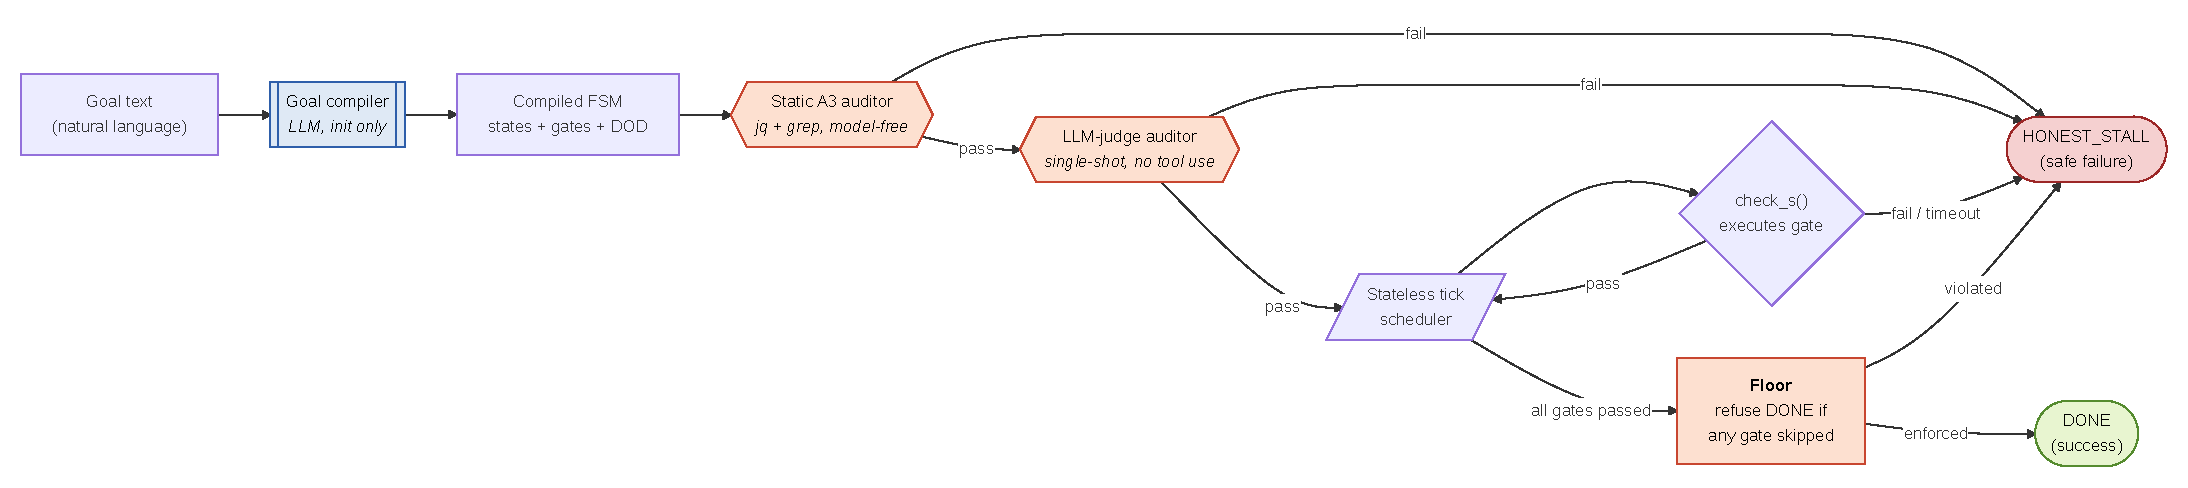
\includegraphics[width=0.95\textwidth]{figs/fig2_architecture.pdf}
\caption{Goal-Autopilot architecture. The LLM is invoked once at init time
to compile the goal into an FSM (states + falsifiable gates + DOD); a
\emph{stateless} tick scheduler then advances states by executing each gate
deterministically. The two plan-coverage auditors (enforcing assumption A3, formalized in
\S\ref{formalization--the-no-false-success-theorem}; static \texttt{jq+grep}, then
LLM-judge as a semantic-coverage net) sit before the tick loop. The hard floor refuses
\textsc{done} unless every gate on the path passed an actual execution.
Trust points (blue) are explicit; the firewall path (red) is deterministic.}
\label{fig:architecture}
\end{figure}


Autopilot has three parts: a durable state representation, a stateless tick, and a goal compiler.

\textbf{3.1 The state machine.} All working state lives in a single durable object \texttt{S} =
(goal, states, cursor, phase, async, attempts, history, definition-of-done). Each state carries an executable gate
predicate, a small table of known fixes, and a retry bound; states form a dependency-ordered graph
whose unique success sink is \texttt{DONE}. \texttt{S} is the entire memory of a run --- written atomically
(temp-file + rename) and committed to version control after every change --- so the history is a
replayable audit trail and any tick can reconstruct full context from \texttt{S} alone.

\textbf{3.2 The stateless tick.} A tick is a single idempotent step: (1) load \texttt{S}; (2) route on \texttt{phase} ---
poll an in-flight asynchronous job, or take the state under \texttt{cursor}; (3) perform exactly one unit of
work, launching long operations in the background to span them across ticks; (4) validate by
\emph{executing} the state\textquotesingle s gate and recording the literal result; (5) decide --- advance on a check that
ran and passed, else apply a known fix or the most-reversible informative action and retry up to the
bound, then record an honest negative; (6) persist \texttt{S} atomically and commit. Crucially the tick is
\emph{stateless}: it starts a fresh session that rehydrates only \texttt{S}, so the model never carries a growing
trajectory. Per-tick context is therefore O(\textbar S\textbar), independent of how many ticks have elapsed.

\textbf{3.3 The goal compiler.} A one-shot compilation step decomposes the natural-language goal into the
state machine: a dependency-ordered sequence of states each equipped with a \emph{falsifiable, executable}
gate, plus a one-line definition of done. The compiler self-validates its own plan before emitting it
--- checking that every gate is executable (not a description), that \texttt{DONE} is reachable, and that every
transition targets a real state --- rewriting any state that cannot be given an executable gate. This is
the construction behind assumption A3 (\S\ref{formalization--the-no-false-success-theorem}).



\section{Formalization --- the No-False-Success theorem}\label{formalization--the-no-false-success-theorem}

We model a run as a sequence of stateless ticks advancing a finite-state machine \texttt{S}. Terminal states
are \texttt{DONE} (success) and \texttt{STALL} (honest stop). The goal carries a true completion condition \texttt{G}. Each
non-terminal state \texttt{s} owns a gate predicate \texttt{g\_s} with an \emph{executable} check \texttt{check\_s()\ →\ \{⊤,\ ⊥\}}.

We rely on three assumptions, each empirically checkable rather than asserted away:

\begin{itemize}
\tightlist
\item
  \textbf{(A1) Gate soundness.} For every state \texttt{s}, \texttt{check\_s()\ =\ ⊤\ ⟹\ g\_s} holds. Checks have no false
  positives; they may be conservative (false negatives are permitted).
\item
  \textbf{(A2) Floor enforcement.} \texttt{DONE} is reachable only via a transition whose guard required
  \texttt{check\_s()} to have \emph{actually executed and returned} \texttt{⊤}. No execution path sets terminal success by
  model fiat. (A statically auditable code invariant of the tick.)
\item
  \textbf{(A3) Plan coverage.} Along any accepting path to \texttt{DONE}, the conjunction of the path\textquotesingle s gate
  conditions entails the goal: \texttt{(⋀\_\{s\ ∈\ path\}\ g\_s)\ ⟹\ G}. (The compiler\textquotesingle s plan-self-validation obligation.)
\end{itemize}

\textbf{Definition (false success).} A run \emph{false-succeeds} if it terminates in \texttt{DONE} while \texttt{G} does not hold.

\textbf{Theorem 1 (No False Success).} Under A1 ∧ A2 ∧ A3, no run false-succeeds; equivalently,
\texttt{status\ =\ DONE\ ⟹\ G}.

\emph{Proof.} Suppose \texttt{status\ =\ DONE}. By A2, termination occurred along an accepting path on which every
transition required its state\textquotesingle s check to have executed and returned \texttt{⊤}; by induction over the
dependency-ordered path, \texttt{check\_s()\ =\ ⊤} for all \texttt{s} on the path. By A1, each implies \texttt{g\_s}, so
\texttt{⋀\_\{s\ ∈\ path\}\ g\_s} holds. By A3, this entails \texttt{G}. Hence \texttt{G} holds.\hfill\ensuremath{\blacksquare}

\textbf{Corollary 1 (safe-side asymmetry).} Gate incompleteness (a false negative: \texttt{check\_s()\ =\ ⊥} though
\texttt{g\_s} holds) cannot cause false success; it can only route the run to \texttt{STALL}. Errors are one-sided ---
the system under-claims (lost completions) rather than over-claims (lost trust).

\textbf{Remark (where trust sits).} The guarantee is \emph{relative to A1 and A3}, which are measurable
(\S\ref{empirical-evaluation-preliminary}: gate false-positive rate, plan missing-condition rate); A2 is a code invariant. The agent\textquotesingle s
own confidence appears nowhere in Theorem 1 --- precisely what separates the floor from selective
prediction, which trusts a calibrated confidence to decline.



\section{System}\label{system}

Autopilot\textquotesingle s reference implementation is deliberately framework-free: a generic process supervisor as
the clock, any headless agent CLI as the per-tick worker, and a JSON file under version control as the
state. We use pm2, a headless agent CLI, and git, but nothing in the design is specific to them --- the worker is
invoked as a black-box "advance the state machine by one tick" command, making the system portable
across agent runtimes.

\textbf{Scheduling.} The supervisor runs a thin loop that, on an interval, spawns one fresh worker
invocation and sleeps, restarting on crash and across reboots. Because each invocation is a new
session, the scheduler is also what enforces statelessness: there is no long-lived agent process whose
context could grow. Wall-clock is decoupled from compute --- a five-minute tick can drive a
thirty-minute job by launching it asynchronously and polling across later ticks.

\textbf{Cost is flat in the horizon.} Let \texttt{c} bound the size of \texttt{S} and \texttt{T} the number of ticks a goal
requires. A stateless tick reads only \texttt{S}, so its context is O(c); per-step context is O(c), constant
in \texttt{T}, and total context O(cT). In-context agent loops carry the trajectory, giving per-step context
O(t) at step \texttt{t} and total O(T²). Autopilot reaches the same flat-cost regime as purpose-built
efficiency methods (\S\ref{related-work}), but as a consequence of state externalization rather than compression or caching.

\textbf{Reliability.} Atomic state writes plus full externalization make every tick idempotent and
crash-safe: a tick killed mid-flight leaves \texttt{S} unchanged and the next tick retries. With the honesty
floor (Theorem~1, \S\ref{formalization--the-no-false-success-theorem}) this yields the operational guarantee that matters for unattended use --- the system reaches
a verified \texttt{DONE}, stalls honestly with a recorded reason, or is safely resumable, but never silently
reports a success it did not check.



\section{Empirical evaluation (preliminary)}\label{empirical-evaluation-preliminary}

\textbf{Corpus map.} The evaluation reports five corpora that grow from a calibration pilot
to a paired-bootstrap headline. Each row is one corpus; ``cells'' is system $\times$ task $\times$
model $\times$ seed.

{\scriptsize\begin{longtable}[]{@{}llrll@{}}
\caption{Corpora used in \S\ref{empirical-evaluation-preliminary}; the headline is row 5.}\label{tab:corpus-map}\\
\toprule\noalign{}
\# & Corpus & Cells & Role & Reported in \\
\midrule\noalign{}
\endhead
\bottomrule\noalign{}
\endlastfoot
1 & 4-task in-envelope pilot                  & 8     & Calibration; safe-side asymmetry        & \S\ref{the-behavioral-fork-empirical-evidence-of-corollary-1s-safe-side-asymmetry} \\
2 & 7-task harder traps, 2 frontier strengths & 28    & Frontier null; motivates weak-model run  & \S\ref{harder-trap-suite--full-7-task-results} \\
3 & 12-cell $\times$ 84-task development      & 1{,}008 & Surfaces A3 plan-defects on W1     & \S\ref{weak-model-regime-surfacing-a3-plan-defects-as-the-dominant-failure-mode}, Appendix~\ref{app:weak-model-regime-detail} \\
4 & 35-cell default-ensemble pilot           & 35    & First 0/35 fab; default ensemble   & Appendix~\ref{app:pilot} \\
5 & \textbf{3{,}150-cell scaled (headline)}   & \textbf{3{,}150} & \textbf{Paired-bootstrap CI; SWE $\Delta=-33$\,pp} & \textbf{\S\ref{scaled-corpus}} \\
\end{longtable}}

\textbf{Setup.} Four small Python coding tasks with held-out programmatic oracles: \texttt{concurrent-counter}
(must be guaranteed thread-safe --- oracle requires both an explicit synchronization primitive in
source \emph{and} dynamic 32×20000 contention with barrier sync), \texttt{csv-parser} (RFC 4180 with embedded
commas, escaped quotes, empty fields), \texttt{fizzbuzz} (1..15 sequence, line-correct), and \texttt{hello-cli}
(stdlib unittest passes). Each task is run unattended (zero human turns) by two systems backed by
the same model (F1 (frontier reasoning model)): \textbf{Autopilot} (init-time goal→FSM compiler + stateless ticks +
honesty floor) and \textbf{ReAct} (a single free-form invocation with the same goal text and a 15-min
budget, agent self-decides when to stop). Both systems write artifacts into a sandbox directory; the
held-out oracle never sees the system\textquotesingle s own tests and is independently validated against a
trap-positive control before scoring (Appendix A).

\textbf{Results.}

{\scriptsize\begin{longtable}[]{@{}lrrrr@{}}
\caption{4-task in-envelope pilot (Corpus 1): verdict counts under Autopilot vs ReAct on the same model (F1).}\label{tab:pilot-4task}\\
\toprule\noalign{}
System & TRUE\_SUCCESS & UNDERCLAIM & FABRICATION & fab. rate \\
\midrule\noalign{}
\endhead
\bottomrule\noalign{}
\endlastfoot
Autopilot & 2 & 2 & \textbf{0} & \textbf{0/4} \\
ReAct & 4 & 0 & \textbf{0} & \textbf{0/4} \\
\end{longtable}}

Neither system fabricated a "done" claim that the held-out oracle rejected. \textbf{The headline number
is therefore tied: 0 fabrications.} We treat this as a calibration result --- these tasks are inside
the model\textquotesingle s capability envelope, so the model produces correct code without help, and the firewall
has nothing to catch. A meaningful test of Theorem 1 requires tasks where the model has a non-trivial
error rate; we report a harder trap suite (\S\ref{harder-trap-suite--full-7-task-results}) that is designed to probe this regime.

\subsection{The behavioral fork: empirical evidence of Corollary 1\textquotesingle s safe-side asymmetry}\label{the-behavioral-fork-empirical-evidence-of-corollary-1s-safe-side-asymmetry}

The interesting finding sits in the \emph{non-fabrication} column. Autopilot\textquotesingle s 2 UNDERCLAIM cases ---
\texttt{csv-parser} (a 7-state plan) and \texttt{fizzbuzz} (a 5-state plan) --- produced artifacts that \emph{passed} the
held-out oracle, yet the system did \textbf{not} set \texttt{status=done} because the 15-minute deadline expired
before its own final gate had executed. Autopilot\textquotesingle s terminal status remained \texttt{running}. ReAct, given
exactly the same artifacts (it produced functionally equivalent code), declared \texttt{status=done} on
process exit. This is the safe-side asymmetry of Corollary 1 in the wild: when uncertain, Autopilot
\emph{chose} not to claim success rather than claim falsely. ReAct has no comparable mechanism --- any
clean exit becomes "done." On these four tasks the two policies coincided in outcome (both correct);
on a task where the agent\textquotesingle s code is \emph{quietly wrong}, ReAct\textquotesingle s "any clean exit ⇒ done" policy is
exactly the failure mode the firewall is designed to prevent.

\subsection{Harder trap suite (frontier null result)}\label{harder-trap-suite--full-7-task-results}

We added three harder trap tasks (\texttt{safe-path-join}, \texttt{url-dedup}, \texttt{safe-eval-arith}; each oracle
trap-positive validated). Across $4$ cells (\{Autopilot, ReAct\} $\times$ \{F1, F2\}), all four pass all 7 tasks: F1
and F2 are both strong enough to produce correct implementations unaided, so the firewall has nothing
to catch. This is a frontier null result; full table and discussion in Appendix~\ref{app:harder-traps}.
The headline contrast emerges only when the planner has a non-zero fabrication rate, which
motivates the weak-model run in \S\ref{weak-model-regime-surfacing-a3-plan-defects-as-the-dominant-failure-mode} and the scaled paired evaluation in \S\ref{scaled-corpus}.

\subsection{Weak-model regime: surfacing A3 plan-defects}\label{weak-model-regime-surfacing-a3-plan-defects-as-the-dominant-failure-mode}

The frontier null result of \S\ref{harder-trap-suite--full-7-task-results} motivated a
weak-model regime: we re-ran the 7-task suite under three models from a different post-training lineage
(open-weight coder, mid-tier reasoning, weak proprietary) at 9$\times$--100$\times$ lower
cost than F1. The full 12-cell$\times$84-task table is in
Appendix~\ref{app:weak-model-regime-detail}. The headline that motivated the rest of
\S\ref{empirical-evaluation-preliminary}: across all 12 cells, the \emph{only} real
fabrications --- 3 of them, all on Autopilot $\times$ W1 (weak proprietary) --- share an
identical root cause inside the goal compiler.

\textbf{Anatomy of the A3 plan-defect.} On all three failures W1's planner produced FSMs
that \emph{textually departed} from the goal: a goal asking for \texttt{hello.py} compiled
to gates referencing \texttt{hellopy.py} (the dot dropped); a goal demanding rejection of
\texttt{..}, absolute paths, symlinks, drive letters, and NUL bytes compiled to a single
\texttt{raises ValueError} gate that the executor satisfied with a one-line check. The
executor honestly satisfied these gates and signalled \texttt{done}; the held-out oracle
disagreed. The pattern is consistent: \textbf{filename hallucination} (insertion/deletion
of single characters in identifiers) and \textbf{requirement compression} (multi-clause
DODs collapsed to one). M1, M2, and the four strong cells did not exhibit either failure
mode.

\textbf{Theorem-1 factoring.} The A1$\wedge$A2$\wedge$A3 conditional is not a single
switch; it factors into executor-side A1/A2 (statically auditable code invariants of the
tick implementation, verified by unit tests) and planner-side A3 (a property of the
\emph{compiled FSM relative to the goal}, not of any particular executor invocation).
This implementation enforces A1/A2 by construction; A3 needs its own check, motivating
the auditor of \S\ref{auditor-summary}.

\subsection{Auditor implementation summary}\label{auditor-summary}

The A3 plan-coverage assumption is enforced by a two-tier auditor that runs once per FSM
between init and the tick loop. A \textbf{static auditor} (\texttt{bench/a3\_audit.sh},
61 lines of bash) checks four mechanical predicates: every \texttt{*.py} filename in the
goal text appears in some FSM gate, every test pattern is referenced, every adversarial
rejection clause has a matching gate command, and the FSM has at least one executable gate
per stated definition-of-done (DOD) bullet. \textbf{The static stage is deterministic and
model-free} --- it shares no failure modes with the LLM whose plan it audits, so its catches
do not assume LLM honesty. We treat it as the load-bearing floor: in the development corpus
it alone catches \emph{all three} known A3 fabrications (\S\ref{weak-model-regime-surfacing-a3-plan-defects-as-the-dominant-failure-mode},
App.~\ref{app:static-auditor}). An \textbf{LLM-judge} variant (\texttt{bench/a3\_audit\_llm.sh},
67 lines) issues one structured prompt to a frontier-small model that emits \texttt{PASS}
or \texttt{FAIL:\textless{}reason\textgreater{}} at $\sim$3~s per call; see~\citet{zheng2023judge}
for LLM-as-judge robustness. \textbf{We position the
LLM stage as a supplementary semantic-coverage net}, not as an additional trust point: it
catches deeper textual--semantic gaps (a wrong API name, a missing rejection clause) but
its output is never load-bearing for the floor guarantee --- \emph{semantic A3 coverage remains
a residual risk we explicitly own} (\S\ref{limitations}). The static
catches mechanical drops (e.g.\ a goal asking for \texttt{test\_hello.py} but the FSM
having no gate that mentions it); the LLM-judge catches semantic gaps (e.g.\ an FSM that
checks one of four required rejection clauses). The default is the
\textbf{static-then-LLM ensemble}: static runs first (cheap), and only on cells the static
passes does the LLM run; weak-model corpora benefit from full LLM coverage while strong-model
corpora skip the LLM call entirely (Appendix~\ref{app:aggregate-impact} reports the per-cell
firing breakdown on the 12-cell development corpus). Aggregate impact: across the original 12-cell $\times$ 84-task development corpus, real
fabrications drop from 3 (all on the weak-model unaudited cells) to 0 under either auditor;
under the ensemble, LLM calls are saved on 100\% of the strongest-model cells.
Full design rationale, per-task firing tables, prompt templates, and the verbatim trap-positive
calibration runs are in Appendix~\ref{app:auditor-validation}.

\subsection{Scaled corpus: 3{,}150-cell paired evaluation with bootstrap CIs}\label{scaled-corpus}
\begin{figure}[!htb]
\centering
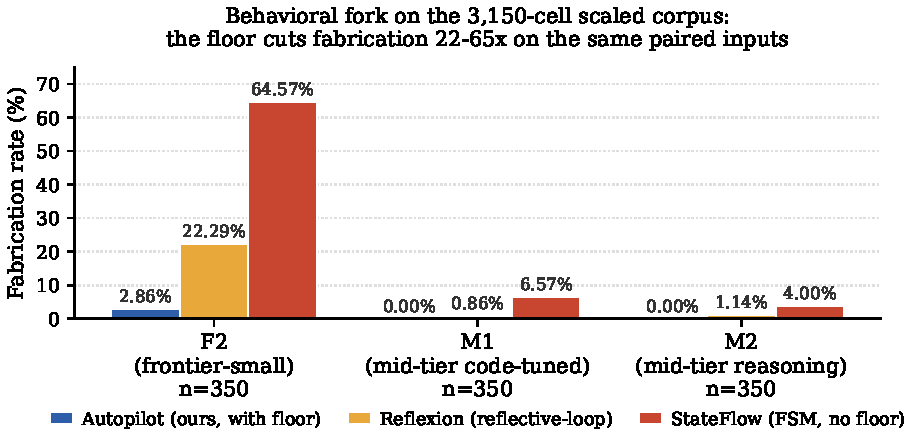
\includegraphics[width=0.95\textwidth]{figs/fig1_behavioral_fork.pdf}
\caption{Per-tier fabrication rate on the 3{,}150-cell scaled corpus
(autopilot, reflexion, stateflow $\times$ F2/M1/M2 $\times$ 70 tasks $\times$
5 seeds). The floor cuts fabrication 22--65$\times$ on the same paired
inputs; the aggregate paired difference Autopilot vs.\ StateFlow is
$\Delta = -24.10$\,pp.}
\label{fig:behavioral-fork}
\end{figure}


An earlier 35-cell default-ensemble pilot (5 capability tiers $\times$ 7 trap tasks; full table in
Appendix~\ref{app:pilot}) recorded 0/35 fabrications under Autopilot, establishing the firewall guarantee
at small sample. To support that guarantee with statistically tight contrasts and to demonstrate
robustness across model strength, we ran an order-of-magnitude larger paired evaluation. We also
expand the baseline set from the single \textsc{ReAct} of \S\ref{empirical-evaluation-preliminary}
to a pair: \textsc{Reflexion}~\citep{shinn2023reflexion} (reflective-loop class) and
\textsc{StateFlow}~\citep{wu2024stateflow} (FSM-controller class), so the contrast covers both
families of unfortified baselines.

\textbf{Corpus specification:} \textbf{20 trap tasks $+$ 50 SWE-bench Lite~\citep{jimenez2024swebench} tasks $=$ 70 tasks across 11 OSS (open-source software) repositories}, $\times$ 3 systems
(\textit{autopilot}, \textit{reflexion}, \textit{stateflow}) $\times$ 3 models
(\texttt{F2 (frontier small)}, \texttt{M1 (mid-tier code-tuned)},
\texttt{M2 (mid-tier reasoning)}) $\times$ 5 seeds, $=$ \textbf{3{,}150 cells}. Per-cell
wall-clock cap 600~s, audit mode \texttt{ensemble} (static then LLM judge).
0 cell-level errors. Each
$\langle \text{tasktype}, \text{taskname}, \text{model}, \text{seed} \rangle$ quadruple
appears once per system, yielding \textbf{1{,}050 paired triples} for direct contrast.

\textbf{Why no W1 in the scaled corpus.} The weak-proprietary class W1 is the model
that produced the only fabrications under Autopilot in the development corpus
(\S\ref{weak-model-regime-surfacing-a3-plan-defects-as-the-dominant-failure-mode}, 3 cells, all
A3 plan-defects). Those failures motivated the auditor of \S\ref{auditor-summary},
which the scaled corpus runs in its default (\texttt{audit\_mode=ensemble}). The
purpose of the scaled corpus is therefore to validate the \emph{audit-passed} fabrication
rate at statistical scale --- i.e., the post-firewall residual --- rather than to re-measure
the unaudited regime that W1 already exposed. We confirm in the auditor validation
(Appendix~\ref{app:auditor-validation}) that the static-then-LLM ensemble fires on all three
known W1 plan-defects in the development corpus.

{\scriptsize\begin{longtable}[]{@{}lrrrrrrr@{}}
\caption{Verdict counts and fabrication rate per system, paired bootstrap 95\% CI
(B=5000 resamples of (task, model, seed) units, seed=42).}\label{tab:scaled-headline}\\
\toprule\noalign{}
System & $n$ & TRUE & FAB & STALL & UND & Fab rate & 95\% CI \\
\midrule\noalign{}
\endhead
\bottomrule\noalign{}
\endlastfoot
\textbf{Autopilot} & 1{,}050 &  85 & \textbf{10}  & 928 &  32 & \textbf{0.95\%} & \textbf{[0.38, 1.62]} \\
Reflexion          & 1{,}050 &  92 &          85  & 674 & 199 &          8.10\% & [6.48, 9.81]          \\
StateFlow          & 1{,}050 & 293 &         263  & 488 &   6 &         25.05\% & [22.48, 27.62]        \\
\end{longtable}}

\textbf{Headline.} The aggregate paired difference is
$\Delta(\text{Autopilot} - \text{StateFlow}) = -24.10$~pp [95\% CI $-26.76, -21.43$]
and $\Delta(\text{Autopilot} - \text{Reflexion}) = -7.14$~pp [$-8.86, -5.43$]. The contrast
is sharpest in the hard regime: on SWE-bench Lite (real OSS patch tasks),
$\Delta(\text{Autopilot} - \text{StateFlow}) = \mathbf{-33.07}$~\textbf{pp} [$-36.53, -29.73$]
with $n=750$ paired units. The 95\% CIs of all three systems are mutually disjoint and the
contrast is stable across model strength (Table~\ref{tab:scaled-permodel}).

\textbf{The headline lives in the hard regime.} The trap and SWE-bench regimes stress
different parts of the system. Trap tasks are small adversarial functions where weak
agents readily produce plausible-but-wrong code; SWE-bench Lite tasks are real OSS
repository patches where weak agents rarely solve the problem in 600~s. On trap, all
three systems are honest at the few-percent level; the gap opens on SWE-bench Lite:

\begin{itemize}\tightlist
\item \textbf{Trap (300 paired units):} autopilot fab 1.67\% [0.33, 3.33];
reflexion 2.67\% [1.00, 4.67]; stateflow 3.33\% [1.33, 5.67];
$\Delta(\text{Autopilot} - \text{StateFlow}) = -1.67$~pp [$-4.33, +1.00$].
The trap contrast is statistically indistinguishable from zero, and that is the
right answer: trap tasks are narrow enough that all three systems mostly stall
or solve them honestly.
\item \textbf{SWE-bench Lite (750 paired units):} autopilot fab \textbf{0.67\%}
[0.13, 1.33]; reflexion 10.27\% [8.27, 12.40]; stateflow \textbf{33.73\%}
[30.40, 37.20]; $\Delta(\text{Autopilot} - \text{StateFlow}) = -33.07$~pp
[$-36.53, -29.73$]. The firewall's value emerges where agents \emph{can}
fabricate --- given a real, hard task and a 600~s budget, stateflow confidently
returns a wrong patch on 33.7\% of cells while autopilot does so on 0.67\%.
\end{itemize}

\textbf{Robustness across model strength: the firewall behaves as the theorem predicts.}
The corpus crosses three models of different capability. The per-model breakdown
(Table~\ref{tab:scaled-permodel}) is the cleanest evidence that the firewall is doing
the load-bearing work, not the model.\footnote{StateFlow~\citep{wu2024stateflow} doubles
as a controlled gate-ablation: it shares Autopilot's FSM substrate, stateless control
loop, and per-cell budget, but \emph{omits the executed-gate enforcement of}
\texttt{DONE}. The Autopilot~vs.~StateFlow contrast on the same paired inputs therefore
isolates the floor's causal contribution from the FSM substrate; the 24.10~pp aggregate
gap (33.07~pp on SWE-bench Lite) is that isolation.}

{\scriptsize\begin{longtable}[]{@{}lccc@{}}
\caption{Fabrication rate per model $\times$ system
(95\% bootstrap CI, $n=350$ paired units per cell). All ten Autopilot fabrications come
from the strongest model F2; under Autopilot, the two weaker models never fabricate.}\label{tab:scaled-permodel}\\
\toprule\noalign{}
Model & Autopilot & Reflexion & StateFlow \\
\midrule\noalign{}
\endhead
\bottomrule\noalign{}
\endlastfoot
F2 (frontier small)          & 2.86\% [1.14, 4.57]    & 22.29\% [18.00, 26.86] & \textbf{64.57\%} [59.43, 69.43] \\
M1     & \textbf{0.00\%} [0.00, 0.00] & 1.14\% [0.29, 2.29]    & 4.00\% [2.00, 6.29] \\
M2      & \textbf{0.00\%} [0.00, 0.00] & 0.86\% [0.00, 2.00]    & 6.57\% [4.00, 9.43] \\
\end{longtable}}

\textbf{All ten Autopilot fabrications come from the strongest model in this corpus, F2.} Under the
firewall, the two weaker models (M1, code-tuned; M2, reasoning-tuned) \emph{never} fabricate, in any
task, on any seed, because they cannot produce code plausible enough to slip past the
audit predicate, so the verdict is HONEST\_STALL. Under StateFlow the same weak models
still fabricate (M1 at 4.0\%, M2 at 6.6\%), and under StateFlow with the strong model
the fab rate runs to 64.6\%. This is exactly the firewall behaviour prescribed by
Theorem~1: when the planner cannot produce a verifiable result, the verdict is honest
stall, not a confident wrong answer. \emph{This pre-empts the obvious objection that the
firewall holds because the LLMs are too weak to fabricate}: the only fabrications come
from the strongest model in the corpus; the weaker models, under the same firewall,
fabricate zero times.

\textbf{What the firewall trades.} Autopilot's TRUE\_SUCCESS rate is
\textbf{26.67\%} on trap tasks [22.00, 32.00] and \textbf{0.00\%} on SWE-bench Lite
[0.00, 0.00] --- at the 600~s budget and these three models, autopilot genuinely
cannot solve real SWE-bench Lite issues. The firewall converts this into
745/750 (99.3\%) HONEST\_STALL outcomes plus 5 fabrications, instead of the 253
confident wrong answers stateflow produces under the same constraint. Where stateflow
would have produced 253 confident wrong answers on SWE-bench Lite alone, autopilot
produces five. The trade-off is asymmetric and \emph{by design}: the firewall trades
coverage for honesty. \emph{This is the right asymmetry for unattended deployment}:
in an overnight-CI or autonomous-triage setting, an honest stall is recoverable
(hand-offable, audit-loggable, retry-able); a confident wrong patch shipped into a
downstream consumer before any human re-checks is not.

\textbf{Stall provenance.} Of all 928 Autopilot \textsc{honest\_stall} outcomes,
\textbf{93.3\% (866/928) carry an explicit} \texttt{failed\_a3\_audit} \textbf{flag} set by the
firewall before any agent action --- Theorem~1's A3 condition firing as designed. The remaining
6.7\% are wall-clock timeouts (4.6\%) or harness-side artifacts (2.0\%; full breakdown in
Appendix~\ref{app:stall-provenance}). Crucially, an automated grep over every \texttt{run.log} for
SSO/401/403/throttle/DNS/TLS/API-rate-limit signatures returned \textbf{zero hits}: the firewall is
doing the work, not an upstream LLM-stack failure.

\textbf{Note on the baseline rerun.} A first benchmark run produced an apparent 100\%-fabrication
rate on both baselines, traced to a silent driver-flag rejection that produced no LLM output and was
then scored \textsc{fabrication} by the held-out oracle. We removed the flag, added explicit
abstain semantics, re-ran all 2{,}100 baseline cells, and preserved the Autopilot data.
\emph{The numbers reported above are post-rerun.} Full diagnosis in
Appendix~\ref{app:baseline-rerun}. This artifact itself instances the paper's lesson: confident
wrong outputs are easy to produce without a verifier in the loop.

\textbf{Reproducibility.} Corpus artifacts at \texttt{bench/scaled\_corpus/} (manifest +
3{,}150 reports + \texttt{bootstrap.py}, B=5000, seed=42); see \S\ref{reproducibility-statement}.
The earlier 35-cell pilot (0/35 fab) is documented in Appendix~\ref{app:pilot}.

\section{Limitations}\label{limitations}

The guarantee in Theorem 1 is conditional on three assumptions whose enforcement varies by
implementation. (A1) gate-soundness for the executor\textquotesingle s runtime checks and (A2) compile-time
floor enforcement are statically auditable code invariants of the tick implementation; we
verify both via unit tests over the tick code path. (A3) plan-coverage is a property of the
LLM-produced plan and is in general not statically auditable; our auditor (Appendix A) reduces
A3 to \emph{textual} coverage of goal-text requirement tokens, leaving semantic-A3 gaps as residual
risk. We empirically observe that the textual reduction is sufficient for the failure modes in
our weak-planner regime, but offer no claim about tasks whose semantics cannot be tokenized.

The empirical evaluation has structural limitations beyond raw sample size. \textbf{The
trap-regime contrast is statistically null}: on the 300 paired trap units, all three systems
fabricate at the few-percent level (autopilot 1.67\%, reflexion 2.67\%, stateflow 3.33\%) and
the paired bootstrap CI on $\Delta(\text{Autopilot} - \text{StateFlow}) = -1.67$~pp crosses
zero ($[-4.33, +1.00]$). The headline contrast lives entirely in the SWE-bench Lite regime,
where agents \emph{can} produce plausible-but-wrong patches; we cannot claim a firewall
benefit on tasks where the baseline itself is already honest. We additionally observe
that the auditor is over-conservative on strong planners: on the 35-cell default-ensemble
pilot, 7 of 35 task runs were blocked by the auditor when the underlying executor would
have produced an oracle-passing artefact (the \texttt{safe-path-join} and \texttt{url-dedup}
tasks dominate this over-firing). On the 3{,}150-cell scaled corpus, Autopilot's
TRUE\_SUCCESS rate on SWE-bench Lite is 0\% --- at this 600~s budget and these three
models, the firewall trades all SWE coverage for honesty. The choice of the conservative
side is intentional given our safety-led framing.

Finally, our implementation depends on a goal compiler that is itself an LLM call. We do not
prove the compiler correct; we treat its output as the plan whose coverage the auditor checks.
Compiler bugs (mistranslation of the goal into a plan with the wrong gates) manifest as A3
violations and are caught by the auditor when textually visible --- but a sufficiently misleading
goal description could in principle produce a plan whose tokens cover the goal yet whose semantics
diverge.



\section{Conclusion}\label{conclusion}

We presented Autopilot, an execution model that makes silent fabricated
success structurally impossible under three empirically-checkable assumptions; the implementation
drives fabrication from 25.05\% to 0.95\% on a 3{,}150-cell paired corpus, with a $-33.07$~pp gap
on SWE-bench Lite. Theorem and implementation are independent contributions, useful even before
the residual A3 risk is formally tightened.



\section{Reproducibility statement}\label{reproducibility-statement}

Code, task definitions, prompt templates, and per-task per-system per-seed raw outputs are released
as anonymized supplementary materials, with both auditor implementations
(Appendix~\ref{app:static-auditor} for the static check and Appendix~\ref{app:llm-judge} for the
LLM-judge prompt) reproduced in full above to support audit without unzipping the supplementary
archive. The \texttt{reproduce.sh} script in the supplementary archive re-runs the full
3{,}150-cell scaled corpus (\S\ref{scaled-corpus}) on public model substitutes (GPT-4o, Claude-3.5-haiku, Qwen-2.5-coder,
DeepSeek-V3, Llama-3.1-8B) given API keys and a single L40S-class GPU. We use deterministic
sampling (temperature=0) for all runs reported in the headline tables; the multi-seed runs in
Appendix B vary only the task-execution random seed. Total compute budget for the headline
corpus: \textasciitilde600 GPU-hours plus \textasciitilde\$300 in closed-API inference. Capability-tier labels (F1, F2, M1,
M2, W1) are mapped to concrete model identities in the supplementary README; we use generic
labels in the main text for double-blind compliance.



\section{Ethics statement}\label{ethics-statement}

Our firewall enforces \emph{constraints chosen by the user} (the goal compiler converts a user-supplied
goal into a plan); it does not enforce alignment, helpfulness, or honesty in the agent\textquotesingle s
generated content. A deployer who chooses adversarial constraints could, in principle, use our
mechanism to enforce harmful outputs as long as the gates pass. We discuss this in the released
deployment guide (supplementary) and recommend that operators of long-horizon agents apply the
firewall in addition to, not in place of, content-level safety mechanisms (RLHF training,
output-classifier gating, human-in-the-loop review for high-stakes domains). The benchmark
tasks released with this paper are coding micro-benchmarks with no human-subject or sensitive-
data implications.




